Natevení filtru typu DP pro \(f_{m} =  \qty{1}{Hz}\) :
\begin{align*}
    \tau &= \frac{1}{\omega} \\
    R\cdot C &= \frac{1}{2\cdot \pi \cdot f_{RC} } \\
    R\cdot C &= \frac{1}{2\cdot \pi \cdot 1 } \\
    R\cdot C &= \num{0.16} \\
\end{align*}

Pokud zvolíme \(R=\qty{1}{M\ohm}\), pro kondenzátor vychází \(C=\num{0.16}/1000 = \qty{160}{nF}\) 

\begin{figure}[h!]
    \centering
    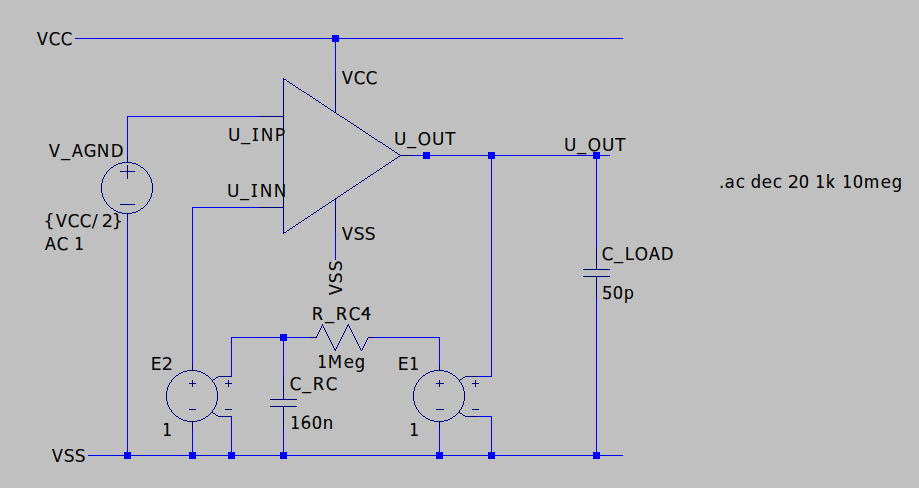
\includegraphics[scale=0.5]{spiceAC.png}
    \caption{Zapojení pro .AC analýzu.}
    \label{fig:spice1.png}
\end{figure}

\begin{figure}[h!]
    \centering
    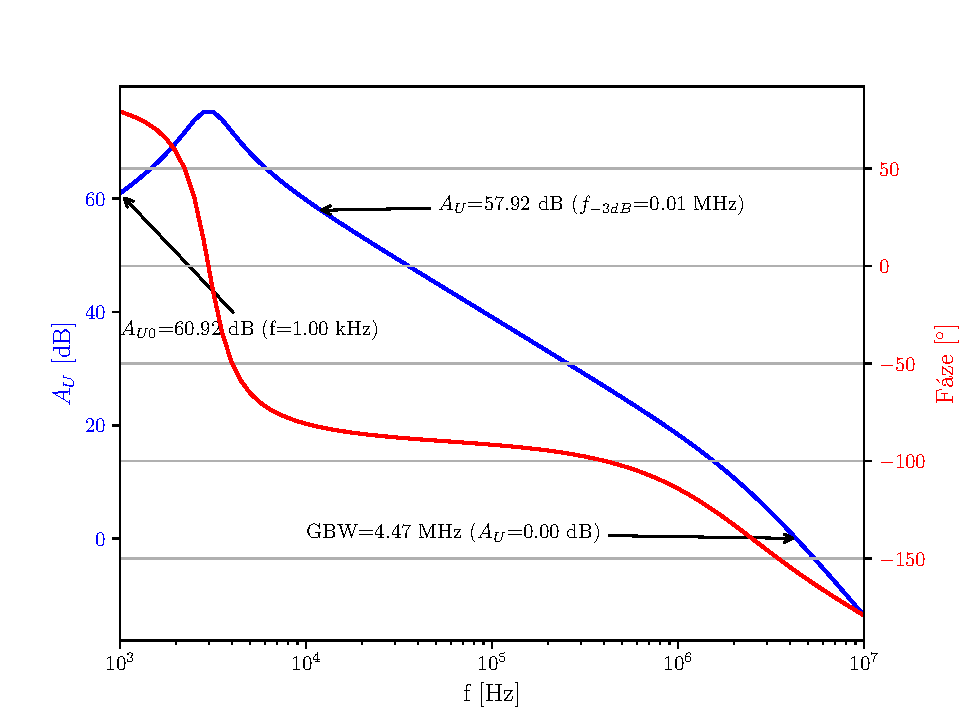
\includegraphics[]{AC.pdf}
    \caption{Výsledky .AC analýzy.}
    \label{fig:spice1.png}
\end{figure}


